\documentclass[
    lithuanian, % Klasei padavus parametrą 'english', darbas bus anglų kalba.
    % signatureplaces % prideda parašų vietas tituliniame puslapyje
]{VUMIFPSkursinis}
\usepackage{float}
\usepackage{wrapfig2}
\usepackage{hyperref}
\usepackage{algorithmicx}
\usepackage{algorithm}
\usepackage{algpseudocode}
\usepackage{amsfonts}
\usepackage{amsmath}
\usepackage{bm}
\usepackage{caption}
\usepackage{color}
\usepackage{graphicx}
\usepackage{listings}
\usepackage{subcaption}
\usepackage{biblatex}
\usepackage{acro}
\usepackage{glossaries}
\usepackage{mathtools}

% https://ctan.math.illinois.edu/macros/latex/contrib/acro/acro-manual.pdf

\acsetup{make-links=true}

\DeclareAcronym{di}{
  short = DI,
  long  = Dirbtinis Intelektas,
  short-plural-form = DI,
  long-plural-form = Dirbtinio Intelekto 
  % highjack plural form for possesive, because plural will never be used
}

\DeclareAcronym{ml}{
  short=ML,
  long={Mašininis Mokymasis},
  extra={\textit{angl. Machine Learning}}
}

\DeclareAcronym{gan}{
  short=GAN,
  long ={Generatyviniai Priešiški Tinklai (\textit{angl. Generative Adversarial Networks})},
  long-plural-form={\textit{angl. Generative Adversarial Networks}}, % highjack plural for english
  extra={generatyviniai varžymosi principais pagrįsti tinklai}
}

\DeclareAcronym{ae}{
  short=AE,
  long={Varžymosi principais pagrįstomis atakomis obfuskuoti kenkėjiško kodo pavyzdžiai (\textit{angl. Adversarial Examples})},
}

\DeclareAcronym{genetic}{
  short=GA,
  long={Genetiniais algoritmais pagrįstas \ac{ml} modelis}
}

\DeclareAcronym{rl}{
  short=RL,
  long={Skatinamasis Mokymasis (\textit{angl. Reinforcement Learning})}
}

\DeclareAcronym{dll}{
  short=DLL,
  long={\textit{angl. Dyanmic-Link Library}}
}

\DeclareAcronym{pe}{
  short=PE,
  long={\textit{angl. Portable Executable}}
}

\DeclareAcronym{nlp}{
  short=NLP,
  long={Skaitmeninis natūraliosios kalbos apdorojimas},
  extra={\textit{angl. Natural Language Processing}}
}

\DeclareAcronym{api}{
  short=API,
  long={\textit{angl. Application Programming Interface}}
}

\DeclareAcronym{svm}{
  short=SVM,
  long={\textit{angl. Support Vector Machine}. TODO}
}

\DeclareAcronym{gbdt}{
  short=GBDT,
  long={\textit{angl. Gradient Boosted Decision Trees}. TODO}
}

\DeclareAcronym{knn}{
  short=KNN,
  long={\textit{angl. $K$-Nearest Neighbours}. TODO}
}

\DeclareAcronym{cnn}{
  short=CNN,
  long={\textit{angl. Convolutional Neural Network}. TODO}
}

\university{Vilniaus universitetas}
\faculty{Matematikos ir informatikos fakultetas}
\department{Programų sistemų studijų programa}
\papertype{Kursinis darbas}
\title{GAN architektūrų, tinkamų kenkėjiško kodo obfuskacijai, analizė}
\titleineng{Analysis of GAN architectures suitable for Ethical Malware Obfuscation}
\author{Liudas Kasperavičius}
\status{4 kurso 3 grupės studentas}
\supervisor{prof. dr. Olga Kurasova}
\reviewer{TBD}
\date{Vilnius – \the\year}

\bibliography{bibliography}
% \glsaddkey
%  {plural-what}% key
%  {}% default value
%  {\glsentryplwhat}% no link cs
%  {\Glsentryplwhat}% no link ucfirst cs
%  {\glsplwhat}% link cs
%  {\Glsplwhat}% link ucfirst cs
%  {\GLSplwhat}% link all caps cs

\glsaddkey{what}% key
{}% default value
{\glsentrywhat}% no link cs
{\Glsentrywhat}% no link ucfirst cs
{\glswhat}% link cs
{\Glswhat}% link ucfirst cs
{\GLSwhat}% link all caps cs

\glsaddkey{whom}% key
{}% default value
{\glsentrywhom}% no link cs
{\Glsentrywhom}% no link ucfirst cs
{\glswhom}% link cs
{\Glswhom}% link ucfirst cs
{\GLSwhom}% link all caps cs
\glsaddkey{whose}% key
{}% default value
{\glsentrywhose}% no link cs
{\Glsentrywhose}% no link ucfirst cs
{\glswhose}% link cs
{\Glswhose}% link ucfirst cs
{\GLSwhose}% link all caps cs

\glsaddkey{plural-whom}% key
{}% default value
{\glsentryplwhom}% no link cs
{\Glsentryplwhom}% no link ucfirst cs
{\glsplwhom}% link cs
{\Glsplwhom}% link ucfirst cs
{\GLSplwhom}% link all caps cs

\glsaddkey{plural-what}% key
{}% default value
{\glsentryplwhat}% no link cs
{\Glsentryplwhat}% no link ucfirst cs
{\glsplwhat}% link cs
{\Glsplwhat}% link ucfirst cs
{\GLSplwhat}% link all caps cs

\newcommand{\glsshort}[1]{\glslink{#1}{\glsentryshort{#1}}}
\newcommand{\Glsshort}[1]{\glslink{#1}{\Glsentryshort{#1}}}

\newglossaryentry{signature}{
    name={Pėdsakas (\angl{Signature})},
    description={Programos struktūros ir požymių santrauka, beveik unikaliai identifikuojanti programą (pvz. \gls{hashfunction})},
    text=pėdsakas,
    first = {pėdsakais \angl{signature}},
}

\newglossaryentry{adversarial}{
    name={Varžymosi principais pagrįstos atakos (\angl{Adversarial Attacks})},
    description={Tai atakos, pritaikytos \enquote{apgauti} \acs{ml} klasifikatorius},
    text=varžymosi principais pagrįstos atakos,
    what=varžymosi principais pagrįstas atakas,
    whom={varžymosi principais pagrįstoms atakoms},
    whose={varžymosi principais pagrįstų atakų},
    first = {varžymosi principais pagrįstoms atakoms \angl{adversarial attacks}},
}

\newglossaryentry{decisionBoundary}{
    name={Sprendimų priėmimo riba (\angl{Decision Boundary})},
    description={Paprasčiausiems \acs{ml} modeliams tai yra kreivė plokštumoje. Sudėtingesniems -- daugiadimensiniams modeliams -- daugdara (\angl{manifold})},
    text=sprendimų priėmimo riba,
    first = {\angl{decision boundary}},
}

\newglossaryentry{zeroSumGame}{
    name={Nulinės sumos žaidimas (\angl{Zero-Sum Game})},
    description={Dviejų žaidėjų žaidimas, kuriame galimas vienas laimėtojas. Laimėtojo laimėta suma yra lygi pralaimėtojo pralaimėtai sumai},
    text={nulinės sumos žaidimas},
    first={nulinės sumos žaidimą \angl{zero-sum game}}
}

\newglossaryentry{surrogateModel}{
    name={Surogatinis Modelis (\angl{Surrogate Model})},
    description={\ac{ml} modelis, aproksimuojantis kitą \ac{ml} modelį, kurio parametrai (svoriai) nėra žinomi},
    text={surogatinis modelis},
    first={surogatinio modelio},
    whom={surogatinio modelio},
    what={surogatinį modelį}
}

\newglossaryentry{policy}{
    name={Strategija (\angl{Policy})},
    description={Tai funkcija $\pi : S \times A \rightarrow \set{0,1}$, čia $S$ -- galimų būsenų erdvė (\angl{State Space}), $A$ -- galimų veiksmų erdvė (\angl{Action Space}). Šią funkciją \acs{rl} modelis \enquote{išmoksta} mokymosi metu},
    text={\angl{policy}}
}

\newglossaryentry{hashfunction}{
    name={Maišymo Funkcija (\angl{Hash Function})},
    description={Tai funkcija $f: \set{0,1}^* \rightarrow \set{0,1}^m$. Naudojama, kai iš begalinės įvesčių erdvės norima gauti fiksuoto dydžio ($m$) išvestį},
    text={maišymo funkcija}
}

\newglossaryentry{framework}{
    name={Karkasas (\angl{Framework})},
    description={Nurodo specifines technologijas, naudojamus požymius ir perturbacijas, siekiamus tikslus \acs{ae} generacijai. Skirtas apibrėžti procesą ir įrankius, kuriuos naudojant būtų galima generuoti nurodytų tikslų siekiančius \acs{ae}},
    text={varžymosi principais pagrįstų atakų karkasas},
    short=karkasas,
    what=karkasą,
    plural=karkasai,
    plural-whom=karkasų,
    plural-what=karkasus,
    whom=karkaso
}

\newglossaryentry{qfunction}{
    name={Q-Funkcija (\angl{Q-Function})},
    description={$Q: S \times A \rightarrow \mathbb{R}$, čia $S$ -- galimų būsenų erdvė (\angl{State Space}), $A$ -- galimų veiksmų erdvė (\angl{Action Space})},
    text=$Q$-funkcija,
    whom=$Q$-funkcijos
}
\makenoidxglossaries{}

\begin{document}

% --------------------------- Citation placeholder ---------------------------

\newcommand{\citeplace}{\textbf{[CITE]}}
\newcommand{\numbers}{\textbf{[NUMBERS NEEDED]}}

\maketitle

\tableofcontents

\sectionnonum{Įvadas}

Pastaraisiais metais kenkėjiškas kodas ir programos kuriamos itin sparčiai (\sim450000 kenkėjiškų programų per dieną \href{https://www.av-test.org/en/statistics/malware/}{AV-TEST} duomenimis). Kenkėjiško kodo aptikimo programos, kurios tradiciškai remiasi programų \gls{signature}, nespėja atnaujinti pėdsakų duomenų bazių pakankamai greitai. Dėl to \acfp{di}, tiksliau Mašininio Mokymosi (\acs{ml}), naudojimas kenkėjiškų programų ar kenkėjiško kodo aptikimo srityje tapo itin populiarus \cite{demetrioAdversarialEXEmplesSurvey2021}. Tačiau \ac{ml} modeliai, nors ir geba aptikti kenkėjiškas programas iš naujų, dar nematytų, duomenų, yra pažeidžiami \gls{adversarial} \cite{castroAIMEDEvolvingMalware2019,huGeneratingAdversarialMalware2017,rosenbergGenericBlackBoxEndEnd2018,zhongReinforcementLearningBased2022}. Šių atakų principas yra \ac{ml} modelio sprendimų priėmimo ribos \gls{decisionBoundary} radimas -- žinant šią ribą pakanka pakeisti kenkėjiškos programos veikimą taip, kad \ac{ml} modelis priimtų sprendimą klasifikuoti ją kaip nekenksmingą \cite{demetrioAdversarialEXEmplesSurvey2021}. Žinoma, rasti šią ribą nėra trivialus uždavinys. Mokslinėje literatūroje išskiriami 3 ribos paieškos atvejai \cite{fangEvadingMalwareEngines2019}:
\begin{enumerate}
    \item \textbf{Baltos dėžės} atvejis: kenkėjiško kodo kūrėjas turi visą informaciją apie \ac{ml} modelį, t.~y. modelio architektūrą, svorius, hiperparametrus.
    \item \textbf{Juodos dėžės su pasitikėjimo įverčiu} atvejis: kenkėjiško kodo kūrėjas gali tik testuoti modelį -- t.~y. pateikti programą ir gauti atsakymą. Atsakymo forma -- klasifikacija ir tikimybė, kad klasifikacija yra teisinga (pasitikėjimo įvertis).
    \item \textbf{Juodos dėžės} atvejis: kenkėjiško kodo kūrėjas gali tik testuoti modelį. Atsakymo forma yra tik klasifikacija.
\end{enumerate}
Akivaizdu, jog \enquote{juodos dėžės} atvejis yra sudėtingiausias, bet ir labiausiai atitinka realias sąlygas \citeplace. Todėl šiame darbe nagrinėjami modeliai, gebantys generuoti varžymosi principais pagrįstų atakų obfuskuotus kenkėjiško kodo pavyzdžius (\acs{ae}) \enquote{juodos dėžės} atvejams.

%  TODO: black box / white box attacks and literature
%  TODO: actualize problem
\vspace{10pt}
\textbf{Tikslas} -- nustatyti labiausiai tinkantį modelį varžymosi principais pagrįstoms atakoms \enquote{juodos dėžės} atvejais.

\vspace{10pt}
\textbf{Uždaviniai}:
\begin{enumerate}
    \item Apžvelgti kenkėjiško kodo obfuskacijos metodus
    \item Nustatyti kriterijus varžymosi principais grįstų atakų modeliams ir juos įvertinti
    \item Atlikti eksperimentinį tyrimą naudojant modelį, gavusį aukštą įvertinimą pagal kriterijus
\end{enumerate}
\section{Literatūros apžvalga}\label{sec:literature}

Mokslinėje literatūroje kenkėjiško kodo ir programų obfuskacijai daugiausia dėmesio skiriama \ac{ae} generavimui, dėl paplitusio \acs{ml} modelių naudojimo kenkėjiško kodo ir programų detekcijos srityje \citeplace. Dažniausia atakų platforma -- operacinė sistema \enquote{Windows} ir jos naudojami \acs{pe} formato failai \citeplace.

Kenkėjiškų programų analizė gali būti išskiriama į \textbf{statinę analizę} ir \textbf{elgesio (\angl{behavior}) analizę}. Statinės analizės detektoriai yra labiau paplitę ir prieinami, kadangi požymių išskyrimas iš tam tikro iš anksto žinomo formato failų ir jų klasifikavimas yra sąlyginai nesudėtinga užduotis. Tuo tarpu elgesio analizės detektoriai dažniausiai neprieinami eiliniams vartotojams, o diegiami korporacijose \citeplace. Jų veikimas pagrįstas nuolatiniu sistemos stebėjimu ir anomalijų detekcija, tad yra kartu ir sudėtingesnė, ir reikalaujanti daugiau resursų, nei statinė analizė, užduotis.

Mokslinėje literatūroje nagrinėjant specifinį būdą generuoti \acs{ae}, apibrėžiamas \gls{framework}. \Glswhat{framework} sudaro
\begin{itemize}
    \item \Glswhom{surrogateModel} tipas ir architektūra
    \item \acs{ml} modelio tipas ir architektūra
    \item \acs{ml} modelio naudojami požymiai (žr. \ref{sec:literature:features})
    \item \acs{ml} modelio naudojamos perturbacijos (žr. \ref{sec:literature:perturbations})
\end{itemize}

\subsection{Naudojami kenkėjiškų programų požymiai}\label{sec:literature:features}
\Gls{adversarial} taikosi į \acs{ml} modeliais paremtus kenkėjiškų programų detektorius. Šie detektoriai yra klasifikatoriai -- pateiktį (programą) klasifikuoja kaip kenkėjišką (\angl{malicious}) arba nekenkėjišką (\angl{benign}). Kadangi programos nėra fiksuoto dydžio, klasifikatoriai remiasi programų požymiais, kurie gaunami atliekant požymių ištraukimą (\angl{feature extraction}). Laikoma, jog \enquote{juodos dėžės} atvejais sužinoti, kokius tiksliai požymius vertina kenkėjiškų programų detektorius, yra neįmanoma, tad \glsplwhom{framework} apibrėžimuose, priklausomai nuo jų specifikos ir tikslų, neretai pateikiami jų vertinami programų požymiai. Šiame poskyryje išskiriami ir klasifikuojami mokslinėje literatūroje minimi požymiai.

\subsubsection{\acs{pe} formato programų požymiai}\label{sec:literature:features:pe}
\begin{itemize}
    \item \textbf{\acs{dll} vardai (arba \acs{api} vardai \cite{huGeneratingAdversarialMalware2017})} \cite{zhongMalFoxCamouflagedAdversarial2024}. \acs{pe} faile turi būti nurodyti visi naudojami \acs{dll} ir jų \acs{api}. Prieš pradedant mokyti \acs{ml} modelį, atliekama visų turimų programų analizė ir nustatoma visų naudojamų \acs{dll} ar jų \acs{api} aibė $D$. Tarkime $|D| = n$. Tuomet, požymių vektorius programai, naudojančiai $X \subseteq D$ \acs{dll}, bus $n$-matis dvejetainis vektorius, kurio $i$-asis elementas yra $\begin{cases}
        0, \text{ jei } D_i \not \in X, \\
        1, \text{ jei } D_i \in X
    \end{cases}$ čia $D_i$ -- $i$-asis $D$ elementas.
    \item \textbf{\acs{pe} metaduomenys} \cite{andersonLearningEvadeStatic2018}. Tai visi \acs{pe} formato faile esantys metaduomenys, tokie, kaip sekcijų pavadinimai, sekcijų dydžiai, \enquote{ImportTable} ir \enquote{ExportTable} metaduomenys ir kt. Formuojant požymių vektorių skaičiuojama metaduomenų \gls{hashfunction}.
\end{itemize}

\subsubsection{Baitų lygio požymiai (gali būti ištraukiami iš bet kokio formato failų)}\label{sec:literature:features:byte}
\begin{itemize}
    \item \textbf{Prasmingų žodžių (angl. Strings) kiekis} \cite{andersonLearningEvadeStatic2018}. Prasmingus žodžius suprantame kaip turinčius prasmę žmogui \textit{(angl. human readable)}. Tai gali būti URL, failų keliai \textit{(angl. file paths)} ar registro raktų pavadinimai. Kadangi prasmingų žodžių kiekis tėra vienas skaičius, požymių vektorius dažniausiai formuojamas prijungiant ir kitus požymius.
    \item \textbf{Baitų/entropijos histograma} \cite{saxeDeepNeuralNetwork2015}. Specifinis metodas, užkoduojantis dažniausiai pasikartojančias baitų ir entropijos poras $n$ dimensijų vektoriumi.
    \item \textbf{$n$-gramos} \cite{zhuNgramMalGANEvading2022}. Dažniausiai sutinkamos skaitmeniniame natūraliosios kalbos apdorojime (\acs{nlp}). Tai yra $n$ žodžių junginiai, arba, sukompiliuotų programų apdorojimo kontekste, $n$ baitų junginiai. Nustatant požymių vektorių, visos $n$-gramos surikiuojamos pagal pasikartojimą programoje mažėjimo tvarka (\enquote{populiariausios} viršuje). Iš pirmų $m$ reikšmių sudaromas $m$-matis vektorius -- tai ir yra požymių vektorius.
\end{itemize}
\subsection{Perturbacijos}\label{sec:literature:perturbations}

Perturbacijos -- tai pagrindinis obfuskacijos metodas \ac{ae} kūrimui.
Perturbacijų tikslas yra pakeisti kenkėjiškos programos veikimą išsaugant
originalų funkcionalumą. Perturbacijos gali būti sudėtingos ir apimti visą
programą (pvz., visos programos užšifravimas ir pridėjimas prie kitos
programos), semantinės (pvz., tam tikrų mašininio kodo instrukcijų keitimas į
ekvivalentų rezultatą pasiekiančias) arba baitų lygio (pvz., nulinių baitų
pridėjimas programos gale) \cite{huGeneratingAdversarialMalware2017}. Perturbacijų parinkimas įeina į
\glswhom{framework} apibrėžimą. Šiame poskyryje aptariamos mokslinėje
literatūroje minimos perturbacijos.
\subsubsection{Baitų lygio perturbacijos}\label{sec:literature:perturbations:byte}
\begin{itemize}
    \item \textbf{\textit{ARBE} (\textit{Append Random Bytes at the End})} \cite{fangEvadingMalwareEngines2019}. \acs{pe} formato failo gale pridedami atsitiktiniai baitai.
    \item \textbf{\textit{ARI} (\textit{Append Random Import})} \cite{fangEvadingMalwareEngines2019}. \acs{pe} formato failo \textit{ImportAddressTable} lentelėje pridedama atsitiktinai pavadinta biblioteka su atsitiktinai pavadinta funkcija.
    \item \textbf{\textit{ARS} (\textit{Append Randomly named Section})} \cite{fangEvadingMalwareEngines2019}. \acs{pe} formato failo \textit{SectionTable} lentelėje pridedamos atsitiktinės sekcijos (sekcijos ir jų tipai yra apibrėžti \acs{pe} formate).
    \item \textbf{\textit{RS} (\textit{Remove Signature})} \cite{fangEvadingMalwareEngines2019}. Sertifikato pašalinimas iš \acs{pe} formato failo \textit{CertificateTable} lentelės.
    \item \textbf{Naujas įeities taškas} \cite{andersonLearningEvadeStatic2018}. Prasidėjus programai, iškart peršokama nuo naujo įeities taško į originalųjį.
    \item \textbf{\textit{Header Fields}} \cite{demetrioAdversarialEXEmplesSurvey2021}. \acs{pe} formato failo \textit{PE Header} ir \textit{Optional Header} dalių specifinių laukų keitimas (pvz., sekcijos pavadinimo keitimas \cite{andersonLearningEvadeStatic2018}).
    \item \textbf{\textit{Partial DOS}} \cite{demetrioAdversarialEXEmplesSurvey2021}. \acs{pe} formato failo \textit{DOS Header} dalies pirmi 58 baitai po \textit{MZ} skaičiaus yra nenaudojami moderniose operacinėse sistemose, tad juos galima keisti.
    \item \textbf{\textit{Slack Space}} \cite{demetrioAdversarialEXEmplesSurvey2021}. Dėl \acs{pe} formato specifikos, kiekviena nauja sekcija turi prasidėti tam tikro skaičiaus, nurodyto \textit{PE Header} dalyje, kartotiniu nuo pradžios. Kompiliatoriai šį reikalavimą išpildo sekcijų gale pridėdami tiek nulinių baitų, kiek reikia teisingam sulygiavimui pasiekti. Būtent ši nulinių baitų erdvė gali būti keičiama be jokios įtakos originaliai programai.
    \item \textbf{\textit{Padding}} \cite{demetrioAdversarialEXEmplesSurvey2021}. Nulinių baitų pridėjimas failo gale.
    \item \textbf{\textit{Full DOS}} \cite{demetrioAdversarialEXEmplesSurvey2021}. Perturbacijos esmė tokia pat, kaip ir \textit{Partial DOS}, tik naudojami visi \textit{DOS} dalies baitai, išskyrus \textit{MZ} ir \textit{PE Offset} (\textit{Partial DOS} manipuliacijoms naudoja tik dalį tarp \textit{MZ} ir \textit{PE Offset}).
    \item \textbf{\textit{Extend}} \cite{demetrioAdversarialEXEmplesSurvey2021}. Pakeičiama \acs{pe} formato faile \textit{DOS} dalyje esanti \textit{PE Offset} reikšmė į didesnę\footnote{\label{footnote:structure}šios reikšmės padidinimas reiškia visos failo struktūros keitimą (\textit{DOS} dalis yra failo pradžioje). Būtina pakeisti visų sekcijų vietas nuo pradžios (\angl{offset}) jų metaduomenyse.}. Taip padidinama (išplečiama) visa \textit{DOS} dalis. Tolesnis perturbacijos principas yra toks pat, kaip ir \textit{Full DOS}.
    \item \textbf{\textit{Shift}} \cite{demetrioAdversarialEXEmplesSurvey2021}. \acs{pe} formato failuose kiekvienas sekcijos blokas prasideda su sekcijos vieta nuo pradžios (\angl{offset}). Tarkime ši reikšmė yra $S$. Sekcijos kodas pradedamas vykdyti tik nuo adreso $P+S$, kur $P$ -- programos pradžios adresas. Vadinasi, padidinus\footnoteref{footnote:structure} $S$ per $n$, atsiranda $n$ baitų laisvos vietos iki sekcijos pradžios, kurią galima keisti be jokios įtakos programos veikimui.
\end{itemize}
\subsubsection{Semantinės perturbacijos}\label{sec:literature:perturbations:semantic}
\begin{itemize}
    \item \textbf{Nereikalingų \hyperref[feature:dll]{DLL/API vardų} požymių pridėjimas} \cite{huGeneratingAdversarialMalware2017}. \acs{pe} formato faile \textit{ImportTable} lentelėje pridedami originalios programos nenaudojami \acs{dll}/\acs{api} vardai.
    \item \textbf{\textit{Binary Rewriting}} \cite{demetrioAdversarialEXEmplesSurvey2021}. Semantinis instrukcijų perrašymas. Pavyzdžiui, $A+B$ instrukcijos pakeitimas į $A-(-B)$.
\end{itemize}

\subsubsection{Kompleksinės perturbacijos}\label{sec:literature:perturbations:complex}
\begin{itemize}
    \item \textbf{\textit{Obfusmal}} \cite{zhongMalFoxCamouflagedAdversarial2024}. Užšifruojama originalios programos kodo sekcija. Sukuriama ir originalios programos gale pridedama programa \textit{Shell.dll}, kurioje laikomas atšifravimo raktas, originalios programos kodo sekcijos adresas ir dydis. Be to, \textit{Shell.dll} geba atšifruoti originalios programos kodo sekciją ir jai perduoti kontrolę. \textit{Shell.dll} pridedama prie naudojamų \acs{dll}, o programos pradžios taškas nustatomas į \textit{Shell.dll} pradžios tašką. Iliustracija pateikiama \ref{fig:perturbations}-ame pav.
    \item \textbf{\textit{Stealmal}} \cite{zhongMalFoxCamouflagedAdversarial2024}. Visa originali programa užšifruojama ir pridedama prie programos \textit{Shell.exe} galo. \textit{Shell.exe} geba atšifruoti originalią programą ir perduoti jai kontrolę. Iliustracija pateikiama \ref{fig:perturbations}-ame pav.
    \item \textbf{\textit{Hollowmal}} \cite{zhongMalFoxCamouflagedAdversarial2024}. Užšifruojama visa originali programa. Ji pridedama prie kurios nors nekenksmingos programos galo. Prie šio junginio galo pridedama \textit{Hollow.dll} programa, kurios veikiamas panašus į \textit{Shell.exe} iš \textit{Stealmal}. Viso junginio pradžios taškas nustatomas į \textit{Hollowmal.dll} pradžios tašką. Iliustracija pateikiama \ref{fig:perturbations}-ame pav.
\end{itemize}

\begin{figure}[h]
    \begin{small}
        \begin{center}
            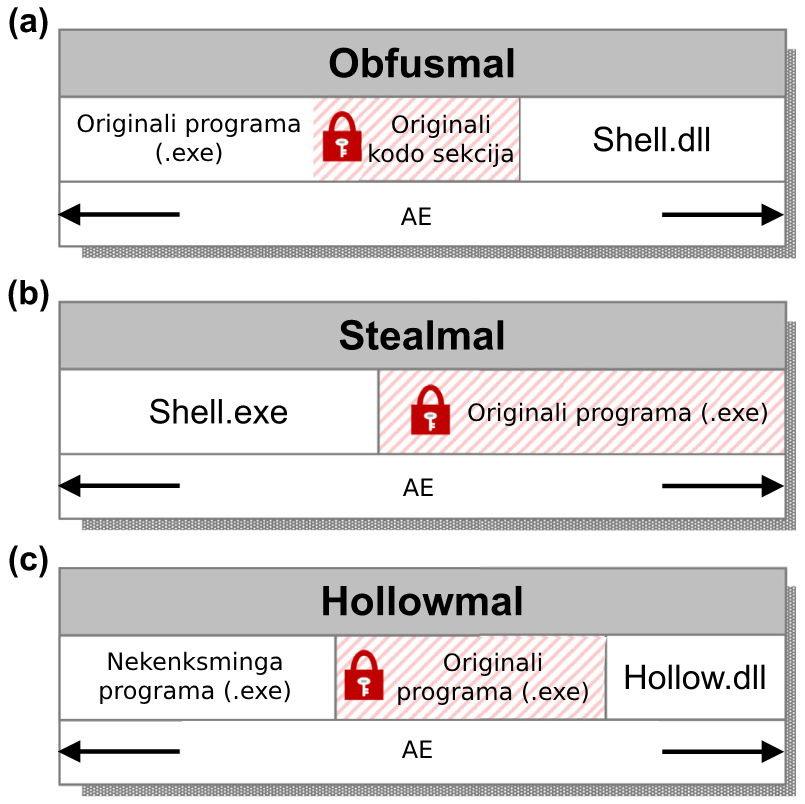
\includegraphics[width=0.95\textwidth]{img/complex-perturbations.png}
        \end{center}
        \caption{Obfusmal (a), Stealmal (b) ir Hollowmal (c) perturbacijų veikimo principų iliustracijos. Adaptuota iš \cite{zhongReinforcementLearningBased2022}}\label{fig:perturbations}
    \end{small}
\end{figure}
\subsection{GAN tipo modelių \glspl{framework}}\label{sec:literature:gan}

\acs{gan} modelių karkasai paremti Generatyviniais Priešiškais Tinklais (\aclp{gan}), kurių veikimo principas yra du neuroniniai tinklai (generatorius ir diskriminatorius), žaidžiantys \gls{zeroSumGame} \cite{chenInfoGANInterpretableRepresentation2016a}. Kenkėjiško kodo obfuskacijos kontekste ir ypač \enquote{juodos dėžės} atvejais, diskriminatorius atlieka \gls{surrogateModel} vaidmenį. Bendras \ac{gan} modelių mokymosi etapas yra tokia seka:
\begin{enumerate}
    \item Generatorius, naudodamas požymių vektorių ir tokios pačios dimensijos
          \enquote{triukšmo} (\angl{noise}) vektorių, sugeneruoja perturbacijas.
    \item Originali kenkėjiška programa modifikuojama pagal perturbacijas (sukuriamas
          \ac{ae}).
    \item Diskriminatorius bando klasifikuoti sugeneruotą \ac{ae} (kenkėjiškas /
          nekenkėjiškas). Diskriminatoriaus klasifikacija lyginama su tikro detektoriaus
          klasifikacija. Jei ji teisinga -- atnaujinami generatoriaus parametrai pagal
          generatoriaus nuostolių funkciją. Kitu atveju, atnaujinami diskriminatoriaus
          parametrai pagal diskriminatoriaus nuostolių funkciją.
    \item Visa seka kartojama nustatytą kiekį kartų.
\end{enumerate} \cite{huGeneratingAdversarialMalware2017,zhuNgramMalGANEvading2022,zhongMalFoxCamouflagedAdversarial2024}.

\begin{describeFramework}{MalGAN}{\cite{huGeneratingAdversarialMalware2017}}
    \introLastPar{
        Tai vienas iš pirmųjų ir populiariausių \acs{gan} tipo modelių \glsplwhom{framework}.
    }
    \purpose{
        Efektyviai išvengti \acs{ae} aptikimo, kai \acs{ml} kenkėjiškų programų detektoriaus implementacija nežinoma (\enquote{juodos dėžės} atvejis)
    }
    \surrogate{
        Daugiasluoksnis tiesioginio sklidimo neuroninis tinklas -- klasifikatorius. Įvestis -- programos požymių vektorius. Išvestis -- klasifikacija į kenksmingą arba nekenksmingą. Šis tinklas taip pat naudojamas kaip diskriminatorius \acs{gan} architektūroje.
    }
    \mainModel{
        Daugiasluoksnis tiesioginio sklidimo neuroninis tinklas. Įvestis -- programos požymių vektorius ir tokios pačios dimensijos \enquote{triukšmo} vektorius. Išvestis -- modifikuotas požymių vektorius. Šis tinklas naudojamas kaip generatorius \acs{gan} architektūroje.
    }
    \features{}{
        \item \textit{MalGan} straipsnyje naudojami tik \acs{api} vardų požymiai, patenkantys į PE formato programų požymių kategoriją (žr. \ref{sec:literature:features:pe}), tačiau autoriai nurodo, jog gali būti naudojami bet kokie požymiai\footnote{\label{footnote:detector-assumptions}autoriai nagrinėja \enquote{juodos dėžės} atvejį su prielaida, jog detektoriaus naudojami požymiai yra žinomi.}.
    }
    \perturbations{}{
        \item Semantinės perturbacijos (\ref{sec:literature:perturbations:semantic}) --
        nereikalingų \acs{api} vardų požymių pridėjimas }
\end{describeFramework}

\begin{describeFramework}{N-gram MalGAN}{\cite{zhuNgramMalGANEvading2022}}
    \introLastPar{
        Šis \glsshort{framework} remiasi \refFramework{MalGAN} karkasu ir siekia jį pagerinti.
    }
    \purpose{
        Supaprastinti, pagreitinti ir pagerinti \glswhat{adversarial}. Pašalinti prielaidas\footnoteref{footnote:detector-assumptions} apie detektorių \enquote{juodos dėžės} atvejais.
    }
    \surrogate{
        Surogatinio modelio veikimas ir architektūra tokia pati, kaip ir \refFramework{MalGAN}
    }
    \mainModel{
        Pagrindinio modelio veikimas ir architektūra labai panašūs į \refFramework{MalGAN}, tačiau norėdami stabilizuoti mokymosi procesą, autoriai siūlo nenaudoti \enquote{triukšmo} vektoriaus. Vietoje to, generatoriaus išvestis ($n$-matis vektorius) modifikuojama nekeičiant pirmų $m$ dimensijų, o kitas $n-m$ pakeičiant nekenksmingų programų požymiais.
    }
    \features{}{
        \item Baitų lygio požymiai (\ref{sec:literature:features:byte}) -- $n$-gramos. }
    \perturbations{Autoriai neatliko eksperimentų su perturbuotomis programomis,
        tačiau pažymi, jog norint gauti sugeneruotus požymių vektorius užtenka pridėti
        reikiamus baitus programos gale. Tai atitinka
        \ref{sec:literature:perturbations:byte} apibrėžtą \vspace{5pt}}{
        \item baitų lygio perturbaciją \textit{ARBE}, tik šiuo atveju pridedami baitai nebūtų
        atsitiktiniai, o norimos $n$-gramos. }
\end{describeFramework}

\begin{describeFramework}{MalFox}{\cite{zhongMalFoxCamouflagedAdversarial2024}}
    \introLastPar{
        \textit{\Name} taip pat remiasi \refFramework{MalGAN}, tačiau siekia kurti \acs{ae} realiomis sąlygomis, dėl to atlieka esminius pakeitimus. 
    }
    \purpose{Generuoti \acs{ae}, kurių neaptiktų komerciniai detektoriai (prieš tai aptarti \glspl{framework} eksperimentams kaip nepriklausomą detektorių naudojo tokius \acs{ml} modelius, kaip \acs{svm}, \acs{knn}, \acs{gbdt} ir kt., bet ne komercinius detektorius). Šio \glswhom{framework} detektorius yra \textit{VirusTotal} (viešai prieinama paslauga, agreguojanti virš 70 komercinių kenkėjiškų programų detektorių).}
    \surrogate{Surogatinis modelis, kaip ir kituose \acs{gan} tipo modelių karkasuose, naudojamas kaip diskriminatorius. Įvestis -- perturbuota programa. Išvestis -- klasifikacija į kenksmingą arba nekenksmingą. Implementacija -- konvoliucinis neuroninis tinklas (\acs{cnn}).}
    \mainModel{Standartinis \acs{gan} generatorius, požymių vektorių sujungiantis su \enquote{triukšmo} vektoriumi. Implementacija -- konvoliucinis neuroninis tinklas (\acs{cnn}).}
    \features{}{
        \item PE formato programų požymiai (\ref{sec:literature:features:pe}) -- \acs{dll}
        vardai. } \perturbations{}{
        \item Visos kompleksinės perturbacijos (\ref{sec:literature:perturbations:complex}) }
\end{describeFramework}
\subsection{Skatinamojo mokymosi tipo modelių karkasai}\label{sec:literature:rl}

Skatinamojo mokymosi (\acs{rl}) modeliai susideda iš agento ir aplinkos. Aplinka susideda iš informatyvių požymių ištraukimo metodo (\textit{angl. feature extraction}) ir kenkėjiškų programų detektoriaus. Agentas -- tai algoritmas ar neuroninis tinklas, kurio tikslas yra surasti optimalią strategiją (\gls{policy}). Šiuo atveju strategija susideda iš perturbacijų (žr. \ref{sec:literature:perturbations}) \citeplace. Bendras \ac{rl} modelių mokymosi etapas yra tokia seka:
\begin{enumerate}
    \item agentas, naudodamas dabartinę aplinkos būseną ir praeito veiksmo atlygį (\textit{angl. reward}), parenka sekantį veiksmą iš galimų veiksmų aibės
    \item atliekamas veiksmas -- perturbuojama programa arba požymių vektorius (priklauso nuo karkaso)
    \item gaunami aplinkos kitimo įverčiai -- nauja būsena ir atlygis, skaičiuojamas pagal detektoriaus klasifikacijos rezultatą
    \item seka kartojama tol, kol agentas nelaiko strategijos optimalia arba nustatytą kiekį kartų
\end{enumerate}
\citeplace{}
\subsection{Genetinių algoritmų tipo modelių \glspl{framework}}\label{sec:literature:genetic}

Genetinai algoritmai (\acs{genetic}) yra viena seniausių mašininio mokymosi
\acs{ml} apraiškų; jų veikimas paremtas evoliucija \cite{castroAIMEDEvolvingMalware2019}. Kenkėjiškų
programų obfuskacijai \acs{ae} generavimas taikant \acs{genetic} yra tokia
seka \cite{yusteOptimizationCodeCaves2022}:
\begin{enumerate}
    \item Sukuriama pradinė populiacija (perturbacijos metodai pradinei populiacijai
          priklauso nuo \glswhom{framework}).
    \item Atliekamas tinkamumo (\angl{fitness}) vertinimas.\label{enum:genetic:fitness}
    \item Atliekama selekcija -- dažniausiai pasirenkami geriausiai įvertinti
          populiacijos \acs{ae}, tačiau galimos ir kitos selekcijos strategijos.
    \item Atliekamas selekcijos atrinktų \acs{ae} kryžminimas (po 2) taip sukuriant naują
          \acs{ae}, turintį po dalį genų iš abiejų kryžmintų \acs{ae}.
    \item Tam tikrai daliai \ac{ae} atliekama dalies genų mutacija.
    \item Vertinama, ar sugeneruoti \acs{ae} atitinka kriterijus (vertina detektorius)
    \item Jei kriterijai nėra tenkinami, seka kartojama nuo \ref{enum:genetic:fitness}-o
          žingsnio.
\end{enumerate}

\begin{describeFramework}{AIMED}{\cite{castroAIMEDEvolvingMalware2019}}
    \purpose{\acs{ae} generavimo greičio padidinimas ir modelių kompleksiškumo sumažinimas, lyginant su \acs{gan} ir \acs{rl} tipo modelių karkasais.}
    \surrogate{Surogatinis modelis nenaudojamas. Naudojami \enquote{juodos dėžės} detektoriai yra \textbf{3 komerciniai} (\textit{Kaspersky, ESET, Sophos}) ir vienas \acs{ml} modelis -- \acs{gbdt}.}
    \mainModel{Klasikinis \acs{genetic} modelis -- veikimas visiškai atitinką bendrą seką. Tinkamumo (\angl{fitness}) vertinamas remiasi \acs{ae} požymių vektoriaus panašumu į originalios programos požymių vektorių (kuo mažiau panašūs, tuo tinkamumo įvertinimas didesnis).}
    \features{}{\item Baitų lygio požymiai (\ref{sec:literature:features:byte}) -- atskiras $n$-gramų
        atvejis, kai $n=1$} \perturbations{}{
        \item Baitų lygio perturbacijos\footnote{autoriai rėmėsi perturbacijomis, aprašytomis
            \cite{andersonLearningEvadeStatic2018}}
        (\ref{sec:literature:perturbations:byte}). }
\end{describeFramework}

\begin{describeFramework}{GAMMA}{\cite{demetrioFunctionalityPreservingBlackBoxOptimization2021}}
    \purpose{Efektyvus (neaptikimo šansų didinmas naudojant perturbacijas, paremtas nekenksmingomis programomis) \glswhose{adversarial} kūrimas.}
    \surrogate{Surogatinis modelis nenaudojamas. \acs{gbdt} ir \textit{MalConv} pasirinkti kaip \enquote{juodos dėžės} detektoriai.}
    \mainModel{Pagrindinė modelio idėja yra požymių ištraukimas iš nekenksmingų programų ir jų pridėjimas, naudojant tam pritaikytas perturbacijas, į kenksmingas programas kiekvienos populiacijos generavimo metu. Tinkamumo (\angl{fitness}) ir kriterijų vertinimas atliekamas naudojant detektorių ir pridėtų požymių dydį baitais (norima pridėti kuo mažiau požymių).}
    \features{}{
        \item \acs{pe} formato programų požymiai (\ref{sec:literature:features:pe}).
        \item Kodas sekcijose (nestandartinis požymis). } \perturbations{}{
        \item Visos baitų lygio perturbacijos (\ref{sec:literature:perturbations:byte}),
        gebančios pridėti baitus.
        \item Autoriai pažymi, jog gali būti naudojama ir \acs{dll} / \acs{api} vardų
        pridėjimo semantinė perturbacija (\ref{sec:literature:perturbations:semantic}).
    }
\end{describeFramework}
\subsection{Nevalidaus PE formato problema}\label{sec:literature:pe_invalid}

Anderson et~al., atlikdami eksperimentus su funkcionalumą išlaikančiomis perturbacijomis \acs{pe} formato failams, pastebėjo, jog ne visais atvejais perturbuotos programos veikia teisingai. Dėl \textit{Windows} operacinės sistemos \acs{pe} formato failų interpretavimo ir paleidimo specifikos, programas įmanoma parašyti tokiu būdu, jog pakeitus kodo ar kitų sekcijų turinį nekeičiant originalių mašininio kodo instrukcijų, programa neveiktų. Techniškai, programų rašymas tokiu būdu pažeidžia patį \acs{pe} formato standartą, tačiau šią praktiką neretai naudoja kenkėjiškų programų autoriai \cite{andersonLearningEvadeStatic2018}.

Norint visiškai išvengti nevalidaus \acs{pe} formato problemos tenka taikyti perturbacijas, nekeičiančias originalių programų, o taikančias kitokius obfuskacijos metodus. Iš \ref{sec:literature:perturbations} poskyryje aptartų perturbacijų, tokias sąlygas atitinka tik 2 kompleksinės perturbacijos (\ref{sec:literature:perturbations:complex}) -- \textit{Stealmal} ir \textit{Hollowmal}.
\section{Modelių vertinimas}\label{sec:criteria}

Modelių vertinimui apibrėšime kriterijus, kurie padės objektyviai išrinkti
realioms \glswhom{adversarial} tinkančius \glsplwhat{framework}. Kriterijus
laikysime esant dviejų tipų: \textbf{kokybiniai} (\glsshort{framework} atitinka
kriterijų arba ne) ir \textbf{kiekybiniai} (\glsshort{framework} atitinka
kriterijų dalinai: 0\% -- visiškai neatitinka, 100\% -- visiškai atitinka). \\

\textbf{Kriterijai} (surikiuoti pagal svarbą mažėjančia tvarka):
\vspace{-5pt}
\begin{enumerate}[label=K-\arabic*., ref=K-\arabic*]
    \item \Glsshort{framework} pritaikytas \enquote{juodos dėžės} atvejams (\textbf{kokybinis}).\label{enum:criteria:blackbox}
    \item \Glsshort{framework} pritaikytas komerciniams detektoriams (\textbf{kokybinis}).\label{enum:criteria:commercial}
    \item \Glsshort{framework} užtikrina realistišką atakos efektyvumo įvertinimą -- naudoja \glswhat{surrogateModel} (\textbf{kokybinis}).\label{enum:criteria:surrogate}
    \item \Glsshort{framework} užtikrina atakos efektyvumą (\textbf{kiekybinis}).\label{enum:criteria:effective}
\end{enumerate}

\newenvironment{criteriaTable}{
    \newcommand{\rowLast}[1]{##1}
    \newcommand{\row}[1]{##1 \\}
    \newcommand{\tbl}[1]{\gdef\Table{##1}}

    \def\Table{}
}{
    \begin{table}[h]
        \centering
        \begin{tabular}{|l|c|c|c|S|}
            \row{
            \textbf{\Glsshort{framework}}           &
            \textbf{\ref{enum:criteria:blackbox}}   &
            \textbf{\ref{enum:criteria:commercial}} &
            \textbf{\ref{enum:criteria:surrogate}}  &
                \textbf{\ref{enum:criteria:effective}}
            } \midrule
            \Table{}
        \end{tabular}
        \caption{\Glsplwhom{framework} vertinimo pagal kriterijus lentelė. \Glspl{framework} surikiuoti pagal įvertinimą mažėjančia tvarka.}
    \end{table}
}

\begin{criteriaTable}
    % \begin{tabular}{cols}
    \tbl{
        \row{ \refFramework{MalFox}        & \cmark{} & \cmark{} & \cmark{} & 56,00\%}
        \row{ \refFramework{MalInfo}       & \cmark{} & \cmark{} & \xmark{} & 59,40\%}
        \row{ \refFramework{AIMED}         & \cmark{} & \cmark{} & \xmark{} & 47,98\%}
        \row{ \refFramework{N-gram MalGAN} & \cmark{} & \xmark{} & \cmark{} & 88,58\%}
        \row{ \refFramework{MalGAN}        & \cmark{} & \xmark{} & \cmark{} & 81,00\%}
        \row{ \refFramework{GAMMA}         & \cmark{} & \xmark{} & \xmark{} & 53,00\%}
        \rowLast{ \refFramework{DQEAF}     & \cmark{} & \xmark{} & \xmark{} & 46,56\%}
    }
    % \end{tabular}
\end{criteriaTable}
\section{Eksperimentinis tyrimas}\label{sec:experiment}

\subsection{Tyrimo aprašymas}
Naudodami \refFramework{MalGAN} \glswhat{framework} paruošime
\glswhat{adversarial} ir apskaičiuosime jų efektyvumą prieš komercinius
detektorius.

\subsubsection{\acs{gan} implementacija} Naudosime \href{https://github.com/ZaydH/MalwareGAN}{viešai
    \textit{Github} platformoje
    paskelbtą\footnote{https://github.com/ZaydH/MalwareGAN}} \textit{MalGAN}
karkaso \acs{ml} modelio implementaciją.

\begin{equation}
    L_{D}= -\mathbb{E}_{x\in BB_{Benign}}\log\left(1-D_{\theta_{d}}(x)\right)\\-\mathbb{E}_{x\in BB_{Malware}}\log D_{\theta_{d}}\left(x\right).\label{eq:LD}
\end{equation}

\begin{equation}
    L_G= \mathbb{E}_{m \in S_{Malware},z \sim p_{\mathrm{uniform} \left[0,1\right) }} \log D_{\theta_d} \left(G_{\theta_g} \left(m,z\right) \right)\label{eq:LG}
\end{equation}

\ref{eq:LD}-oje ir \ref{eq:LG}-oje lygtyse atitinkamai pateikiamos \textit{MalGAN} diskriminatoriaus ir generatoriaus nuostolių funkcijos. Šiose lygtyse naudojamų simbolių prasmės paaiškinimas pateikiamas \ref{tab:eq_explain}-oje lentelėje.

\begin{table}[h]
    \begin{small}
        \begin{center}
            \begin{tabular}[c]{l|p{0.75\textwidth}}
                Simbolis       & Prasmė                                                                                                                                           \\
                \midrule
                $BB_{Benign}$  & Požymių vektorių, kuriuos \enquote{juodos dėžės} detektorius klasifikuoja kaip \textbf{nekenksmingus}, aibė                                      \\

                $BB_{Malware}$ & Požymių vektorių, kuriuos \enquote{juodos dėžės} detektorius klasifikuoja kaip \textbf{kenksmingus}, aibė                                        \\

                $S_{Malware}$  & Tikrų kenkėjiškų programų požymių vektorių aibė                                                                                                  \\

                $D_{\theta_d}$ & Diskriminatorius su $\theta_d$ svoriais ($D_{\theta_d}: \set{0,1}^{n_m} \rightarrow [0,1], \; n_m \in \mathbb{N}$)                               \\

                $G_{\theta_g}$ & Generatorius su $\theta_g$ svoriais ($G_{\theta_g}: \set{0,1}^{n_m} \times {[0,1]}^{n_z} \rightarrow \set{0,1}^{n_m}, \; n_m, n_z \in \mathbb{N}$) \\

                $z$            & Triukšmo vektorius                                                                                                                               \\

            \end{tabular}
        \end{center}
        \caption{\textit{MalGAN} nuostolių funkcijų formulėse naudojamų simbolių paaiškinimas}\label{tab:eq_explain}
    \end{small}
\end{table}


\subsubsection{\acs{gan} mokymosi duomenys} Mokymuisi naudosime \textit{EMBER}
\cite{andersonEMBEROpenDataset2018a} duomenų rinkinį. Treniravimo aibė susideda
iš $2000$ programų požymių (\textit{API} vardų iš \textit{ImportTable} \acs{pe}
formato failo sekcijos). Aibė subalansuota -- joje yra po $1000$ kenkėjiškų ir
nekenkėjiškų programų požymių. Mokymosi etapui taip pat taikysime treniravimo /
validacijos skaidinį santykiu $4:1$.

\subsubsection{\Glswhom{framework} parametrai}

Tyrimo metu atlikti 2 eksperimentai (\textbf{E-1} ir \textbf{E-2}), kuriems
parinkti \ref{tab:experiment:params}-oje lentelėje aprašyti parametrai.
\textbf{E-1} atitinka \textit{MalGAN} straipsnyje
\cite{huGeneratingAdversarialMalware2017} aprašytą eksperimentą, \textbf{E-2}
-- eksperimentas su autoriaus parinktais parametrais siekiant padidinti atakų
efektyvumą.

\begin{table}[h]
    \begin{tabular}{|l|l|l|}
        \textbf{Parametras}                                                   & \textbf{E-1} & \textbf{E-2}       \\
        \midrule
        Dvejetainio požymių vektoriaus $M$ dimensija                          & 160          & $10000$            \\
        \enquote{Triukšmo} vektoriaus $Z$ dimensija                           & 10           & $100$              \\
        Neuronų skaičius generatoriaus \enquote{paslėptuose} sluoksniuose     & 256          & $100,256,512,1024$ \\
        Neuronų skaičius diskriminatoriaus \enquote{paslėptuose} sluoksniuose & 256          & $256,256$          \\
        Diskriminatoriaus mokymosi greitis                                    & $10^{-3}$    & $4\cdot 10^{-4}$   \\
        Generatoriaus mokymosi greitis                                        & $10^{-3}$    & $10^{-6}$          \\
    \end{tabular}
    \caption{Eksperimentuose naudoti \acs{ml} modelio parametrai}\label{tab:experiment:params}
\end{table}

\subsubsection{Realių kenkėjiškų programų rinkinys}\label{sec:experiment:virusshare}
Atakoms naudosime realias kenkėjiškas \acs{pe} formato programas iš
\href{https://virusshare.com/}{\textit{VirusShare}\footnote{https://virusshare.com/}}.
Duomenų rinkinį sudaro $100$ kenkėjiškų programų.

\subsubsection{Komerciniai detektoriai}
Tiek originalias, tiek modifikuotas (\acs{ae}) kenkėjiškas programas
patikrinsime su
\href{https://www.virustotal.com}{\textit{VirusTotal}\footnote{https://www.virustotal.com}}
-- paslauga, kuri agreguoja daugiau nei $70$ komercinių kenkėjiškų programų
detektorių.

\clearpage
\subsection{Mokymosi etapas}

Specifinis \refFramework{MalGAN} mokymosi etapas yra tokia seka:
\begin{enumerate}
    \item Išmokomas \enquote{juodos dėžės} modelis (šiuo atveju pasirinktas
          \enquote{atsitiktinio miško} (\angl{random forest}) modelis).
    \item Mokoma pagal bendrą seką (aptartą \ref{sec:literature:gan}), kurioje:
          \begin{itemize}
              \item Praleidžiamas originalios programos perturbacijos žingsnis (diskriminatoriui
                    iškart perduodamas \acs{ae} požymių vektorius).
              \item Generatorius ir diskriminatorius mokomi kartu, kadangi diskriminatorius turi
                    naudoti generatoriaus sugeneruotus \acs{ae}, o generatoriaus nuostolių funkcija
                    priklauso nuo diskriminatoriaus išvesties. Šis žingsnis pavaizduotas
                    \ref{fig:experiment:learning:combined}-ame pav.
          \end{itemize}
\end{enumerate}

\begin{figure}[h]
    \begin{small}
        \begin{center}
            \begin{subfigure}[t]{0.5\textwidth}
                \centering
                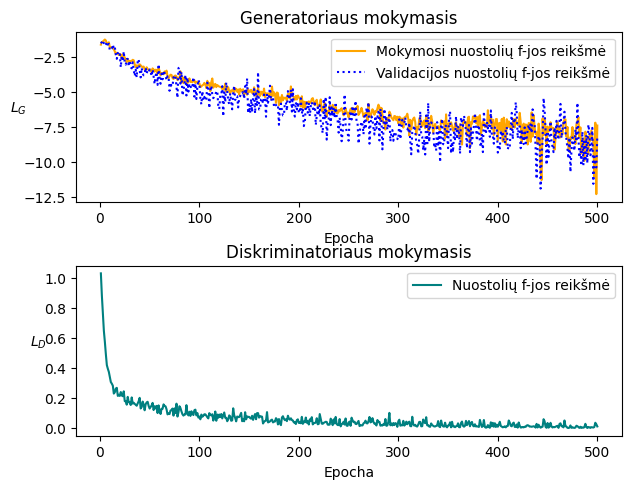
\includegraphics[width=\textwidth]{img/learning_paper.png}
                \caption{\textbf{E-1}}\label{fig:experiment:learning:paper}
            \end{subfigure}
            \hfill
            \begin{subfigure}[t]{0.48\textwidth}
                \centering
                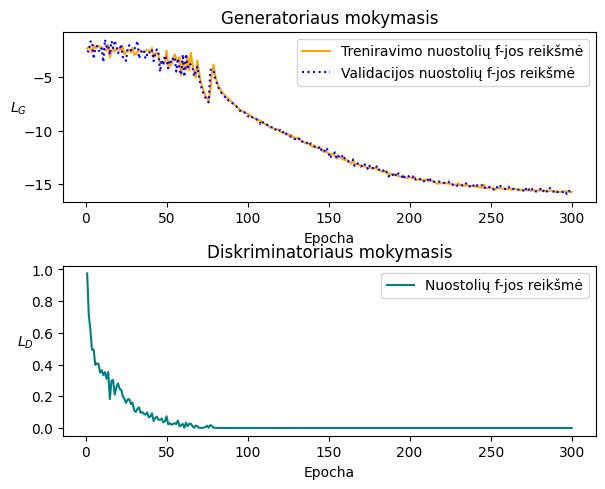
\includegraphics[width=\textwidth]{img/learning.png}
                \caption{\textbf{E-2}}\label{fig:experiment:learning}
            \end{subfigure}
        \end{center}
    \end{small}
    \caption{\textit{MalGAN} generatoriaus ir diskriminatoriaus nuostolių funkcijų reikšmės mokymosi etape}\label{fig:experiment:learning:combined}
\end{figure}

\clearpage
\subsection{Varžymosi principais pagrįstos atakos prieš komercinius detektorius}

Naudodami mokymosi etape ištreniruotą \acs{ml} modelį ir
\ref{sec:experiment:virusshare} aptartą duomenų rinkinį, sugeneruosime \acs{ae}
ir palyginsime, kiek komercinių detektorių aptinka originalias programas
($N_{orig}$) ir kiek obfuskuotas pagal \textit{MalGAN} karkasą ($N_{adv}$).

Atakų efektyvumą $\mu$ skaičiuosime remiantis Zhong et~al. pasiūlyta formule
$\mu' = \frac{N_{orig} - N_{adv}}{N_{orig}}$
\cite{zhongMalFoxCamouflagedAdversarial2024}. Eksperimentuose galimi atvejai,
kai originalią programą aptinka mažesnis detektorių kiekis, nei obfuskuotą
($N_{orig} < N_{adv}$). Tokiais atvejais $\mu' < 0$. Kadangi neigiamas atakos
efektyvumas neturi prasmės, laikome, jog atvejais, kai $\mu' < 0$ ataka nėra
efektyvi (t.~y. jos efektyvumas lygus $0$) $\implies$ $\mu = \max{(\mu', 0)}$.

Atakų efektyvumų pasiskirstymas pavaizduotas \ref{fig:experiment:mu_dist}-ame
pav., tarpiniai rezultatai ($N_{orig}$ ir $N_{adv}$), naudojami pasiskirstymų
skaičiavimui pateikiami \ref{fig:experiment:det_dist}-ame pav.
(\ref{app:experiment}-ame priede).

\begin{figure}[h]
    \begin{small}
        \begin{center}
            \begin{subfigure}[t]{0.48\textwidth}
                \centering
                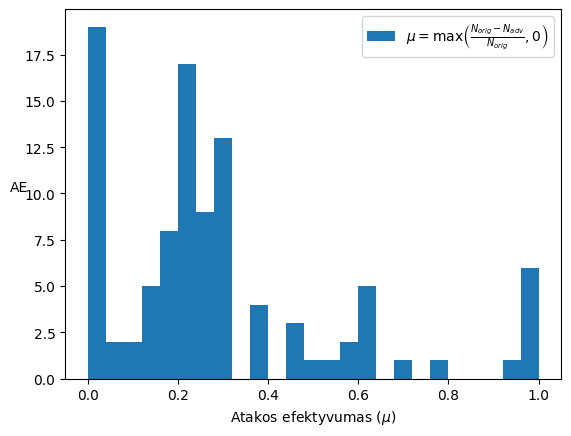
\includegraphics[width=\textwidth]{img/mu_distribution_paper.png}
                \caption{\textbf{E-1}}
            \end{subfigure}
            \hfill
            \begin{subfigure}[t]{0.48\textwidth}
                \centering
                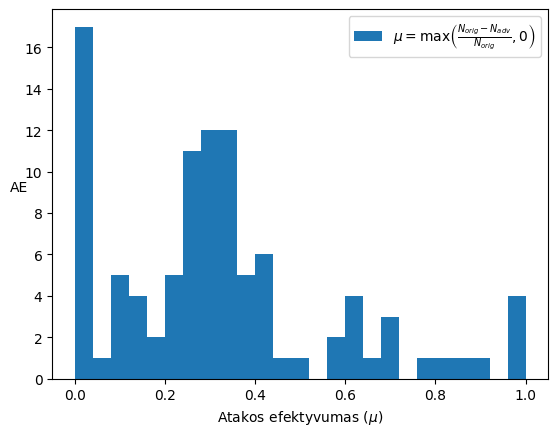
\includegraphics[width=\textwidth]{img/mu_distribution.png}
                \caption{\textbf{E-2}}
            \end{subfigure}
        \end{center}
        \caption{\Glswhose{adversarial} efektyvumo prieš komercinius detektorius pasiskirstymas}\label{fig:experiment:mu_dist}
    \end{small}
\end{figure}

Tyrimo apibendrinimui \ref{tab:experiment:stats}-oje lentelėje pateikiamos
abiejų eksperimentų statistikos, apskaičiuotos iš
\ref{fig:experiment:mu_dist}-ame pav. vaizduojamų duomenų įtraukiant ir
neefektyvias atakas (kai $\mu = 0$).

\begin{table}[h]
    \centering
    \begin{tabular}{l|l|l}
                                                   & \textbf{E-1} & \textbf{E-2} \\
        \midrule
        \textbf{Efektyvumo vidurkis ($\bar{\mu}$)} & $28,89\%$    & $26,85\%$    \\
        \textbf{Standartinis nuokrypis ($\sigma$)} & $26,31\%$    & $18,97\%$    \\
    \end{tabular}
    \caption{Eksperimentų statistikos}\label{tab:experiment:stats}
\end{table}

\sectionnonum{Rezultatai ir išvados}

\subsection*{Rezultatai}
\begin{enumerate}
    \item Išanalizuoti 8 trims kategorijoms (\acs{gan}, \acs{rl}, \acs{genetic}) priklausantys \glswhose{adversarial} \glspl{framework}. 
    \item Jiems apibrėžti vertinimo kriterijai, išskiriantys geriausiai realioms sąlygoms pritaikytus \glsplwhat{framework}.
    \item Atliktas tyrimas, kurio metu \ref{enum:criteria:commercial} kriterijaus neįgyvendinantis \gls{framework} \refFramework{MalGAN} naudojamas \acs{ae} generavimui prieš komercinius detektorius ir renkami \ref{enum:criteria:effective} kriterijų atitinkantys duomenys (t.~y. nustatomas \glswhom{framework} \ref{enum:criteria:effective} kriterijus tokiomis sąlygomis, kai tenkinamas \ref{enum:criteria:commercial}).
\end{enumerate}

\subsection*{Išvados}
\begin{enumerate}
    \item Tyrimo metu atlikti 2 eksperimentai parodo, jog net ir padidinus \textit{MalGAN} \acs{ml} modelio galimybes (suteikus daugiau kompiuterijos resursų), atakų efektyvumas prieš komercinius detektorius nepadidėja ($\bar{\mu}_{E \text{-} 2} < \bar{\mu}_{E \text{-} 1}$), tačiau yra stabilesnis ($\sigma_{E \text{-} 2} < \sigma_{E \text{-} 1}$).
    \item Abiem atvejais tyrimo metu gautas \ref{enum:criteria:effective} įvertis ($\bar{\mu}$) yra žymiai mažesnis už kriterijų vertinimo metu naudojamą $81,00 \; \%$ \textit{MalGAN} \glswhom{framework} įvertinimą (kai \ref{enum:criteria:commercial} netenkinamas). Tai paaiškina \ref{tab:criteria}-oje lentelėje matomas \ref{enum:criteria:effective} kriterijaus anomalijas ir parodo, jog kriterijai ir \glsplwhom{framework} vertinimas yra adekvatūs.
    \item Laikant, jog parinkti kriterijai ir jų vertinimas yra patikimi, geriausiai iš analizuotų \glsplwhom{framework} \enquote{juodos dėžės} atvejams pritaikytas \gls{framework} yra \refFramework{MalFox}, tenkinantis visus 3 kokybinius kriterijus ir siekiantis $56,00 \; \%$ kiekybinį įvertinimą (atakų efektyvumą).
\end{enumerate}


\printbibliography[heading=bibintoc]

\sectionnonum{Sąvokų apibrėžimai}
\renewcommand{\glossarysection}[2][]{}
\printnoidxglossary{}

\sectionnonum{Santrumpos}
\printacronyms[heading=none]

\appendix{}
% \appendix{Kompleksinių perturbacijų iliustracijos}
% \begin{figure}[h]
%     \begin{small}
%         \begin{center}
%             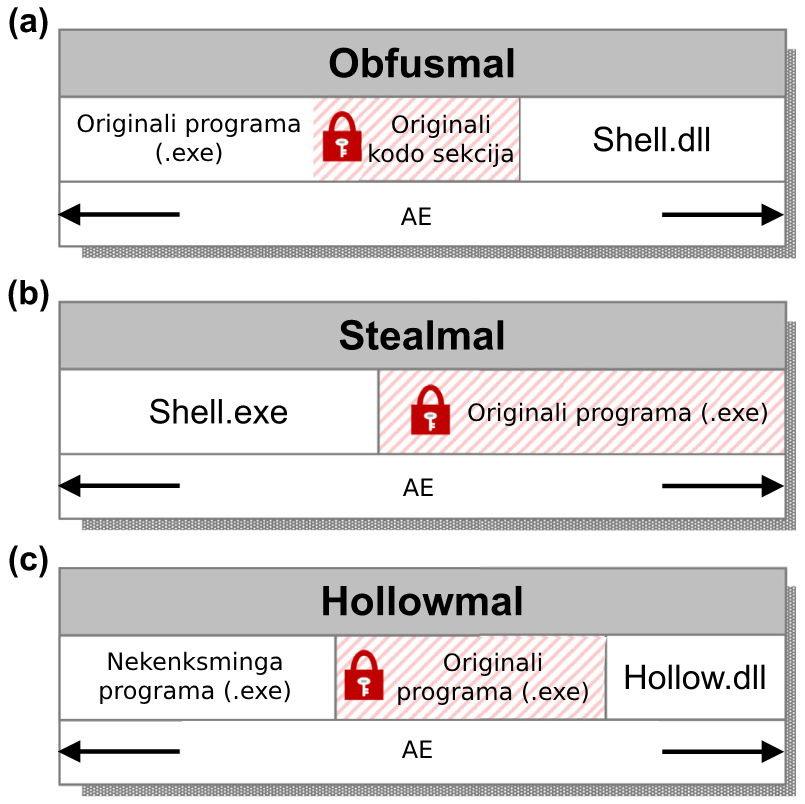
\includegraphics[width=0.95\textwidth]{img/complex-perturbations.png}
%         \end{center}
%         \caption{Obfusmal (a), Stealmal (b) ir Hollowmal (c) perturbacijų veikimo principų iliustracijos. Adaptuota iš \cite{zhongReinforcementLearningBased2022}}\label{fig:perturbations}
%     \end{small}
% \end{figure}

\appendix{Tarpiniai tyrimo rezultatai}\label{app:experiment}
\begin{figure}[h]
    \begin{small}
        \begin{center}
            \begin{subfigure}[t]{0.48\textwidth}
                \centering
                \caption{\textbf{E-1}}
                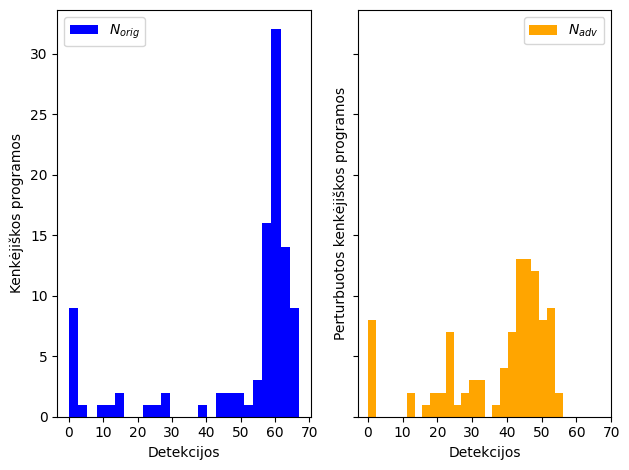
\includegraphics[width=\textwidth]{img/det_distributions_paper.png}
            \end{subfigure}
            \hfill
            \begin{subfigure}[t]{0.48\textwidth}
                \centering
                \caption{\textbf{E-2}}
                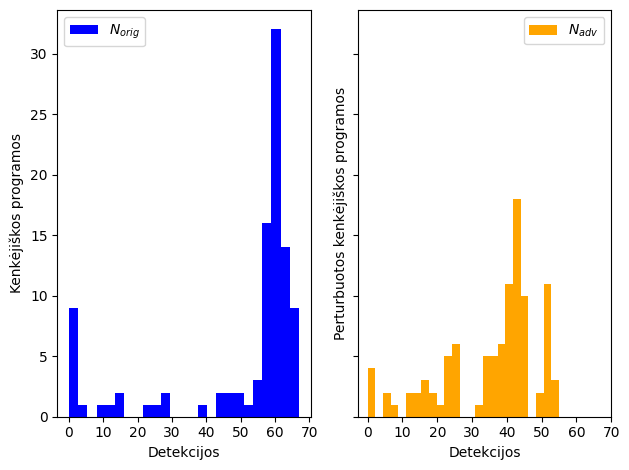
\includegraphics[width=\textwidth]{img/det_distributions.png}
            \end{subfigure}
        \end{center}
        \caption{Originalių ($N_{orig}$) ir perturbuotų ($N_{adv}$) kenkėjiškų programų detekcijų pasiskirstymas}\label{fig:experiment:det_dist}
    \end{small}
\end{figure}

\end{document}
